\documentclass[12pt,a4paper,oneside,onecolumn]{article}

\usepackage[spanish,es-noshorthands]{babel}
\usepackage{epsfig}
\usepackage[latin1]{inputenc}
\usepackage{amsmath}
\usepackage{amsfonts}
\usepackage{amssymb}
%\usepackage{mathabx}  Compila pero borra el pdf?
\usepackage{array}
\usepackage[left=1.8cm, right=1.8cm, top=2.50cm, bottom=2.5cm]{geometry}
\usepackage{hyperref}
\usepackage{color}
\usepackage{fancyhdr}
\usepackage{listings}
\usepackage{xcolor}

\pagestyle{fancy}

\fancyhead{}
\fancyfoot{}

\setlength{\headsep}{0.4cm}
\setlength{\footskip}{1.6pt}
\setlength{\parindent}{0pt}
\setlength{\extrarowheight}{1.5pt}


\lhead{An\'alisis Matem\'atico I}
\rhead{Javier Orti}
\renewcommand*\headrulewidth{0.4 pt}
\lfoot{\vspace{0.45cm}Pr\'actica 2}
\cfoot{\vspace{0.01cm}\rule{\linewidth}{0.4pt}}
\rfoot{\vspace{0.45cm} P\'ag. \thepage}

\renewcommand{\labelitemi}{$\bullet$}
\renewcommand{\labelenumi}{\theenumi)}
\renewcommand\spanishtablename{Tabla}

\decimalpoint

\headheight 16.7pt 
\textheight 715pt 

\parskip 8pt  

\hypersetup{
	colorlinks=true,
	linkcolor=blue,
	filecolor=magenta,      
	urlcolor=cyan,
}

% Python code settings
\definecolor{codegreen}{rgb}{0,0.6,0}
\definecolor{codegray}{rgb}{0.5,0.5,0.5}
\definecolor{codepurple}{rgb}{0.58,0,0.82}
\definecolor{backcolour}{rgb}{0.95,0.95,0.92}

\lstdefinestyle{mystyle}{
	backgroundcolor=\color{backcolour},   
	commentstyle=\color{codegreen},
	keywordstyle=\color{magenta},
	numberstyle=\tiny\color{codegray},
	stringstyle=\color{codepurple},
	basicstyle=\ttfamily\footnotesize,
	breakatwhitespace=false,         
	breaklines=true,                 
	captionpos=b,                    
	keepspaces=true,                 
	numbers=left,                    
	numbersep=5pt,                  
	showspaces=false,                
	showstringspaces=false,
	showtabs=false,                  
	tabsize=2
}

\lstset{style=mystyle}

\begin{document} 
    % Ejercicio 1 %
    \section{}
    \[
        (z -1 -i)(z +1 +i)(z -1 +i)(z +1 -i) = 4 + i
    \]
    \newline Expresamos $a = 1 + i$ y $\Bar{a} = 1-i$ como su conjugado y obtenemos:
    \[
        (z - a)(z + a)(z - \Bar{a})(z +\Bar{a}) = (z^2 - a^2)(z^2-\Bar{a}^2)
    \]
    \[
         (z^2-(1-i^2+2i))(z^2 - (1-i^2-2i))
        = (z^2 - 2i)(z^2 + 2i) =
    \]
    \[
        z^4 - (2i)^2 = 4 + i \xrightarrow[]{} z^4 = i
    \]
    como $i$ forma un angulo $\theta = \pi/2$, su expresion exponencial ser\'a:
    \[
        i = e^{i\pi/2}
    \]
    y por tanto la ecuaci\'on:
    \[
        z = \sqrt[4]{e^{i\pi/2}} = e^{\frac{\pi/2 + 2\pi k}{4}} = e^{\frac{\pi}{8} + \frac{\pi}{2}k}, k \in \mathbb{Z}
    \]
    \begin{figure}[!h]
		\centering
		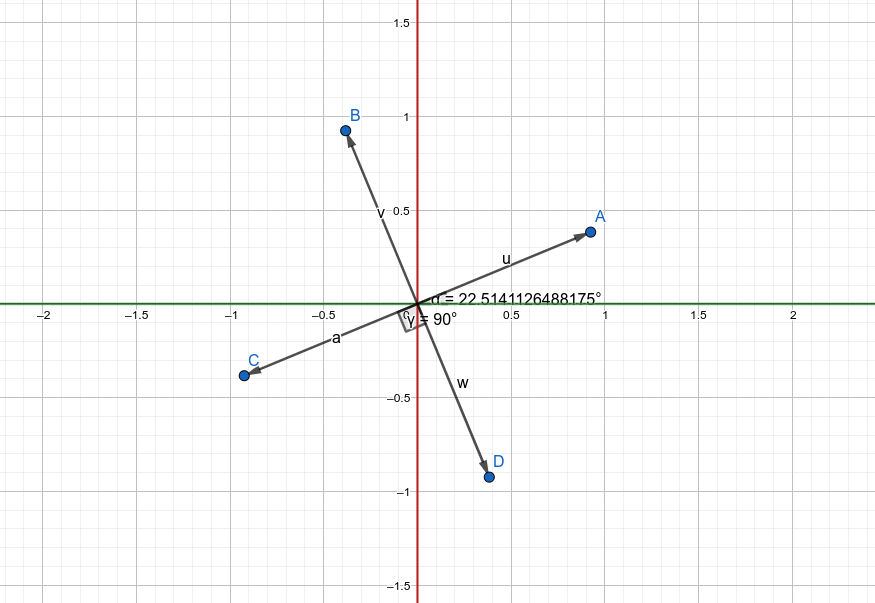
\includegraphics[scale=0.55]{ex1.png}
		\caption{}
		\label{fig:1}
	\end{figure}
    % Ejercicio 2 %
    \newline \newline 
    \section{}
    \[
        \begin{cases}
            (3 - i\ )x + (4 + 2i)y = 2 + 6i \\ 
            (4 + 2i)x - (2 + 3i)y = 5 + 4i
        \end{cases}
    \]
    Resolvemos utilizando la regla de Cramer:
    \[
        A = \begin{pmatrix}
            3 - i & 4 + 2i \\
            4 + 2i & 2 + 3i 
            \end{pmatrix}
    \]
    \[
        A_x = \begin{pmatrix}
            2 + 6i & 4 + 2i \\
            5 + 4i & 2 + 3i 
            \end{pmatrix}
    \]
    \[
        x = \frac{|A|}{|A_x|} = \frac{2 - 44i}{21+23i} = - \frac{(2 - 44i)(21-23i)}{21^2 + 23^2} = -\frac{-970 - 970i}{970}= 1 + i
    \]
    Despejamos la y de la 1a $1^a$ ecuaci\'on y sustituimos:
    \[
        y = \frac{2 + 6i -(3-i)x}{4+2i} = \frac{2 + 6i -3 -3i +i -1}{4 + 2i} = \frac{(-2+4i)(4-2i)}{16 + 4} = i
    \]

    % Ejercicio 3 %
    \section{}
    Para que $\mathbb{C}$ tenga estructura de cuerpo, debe cumplir que $ \mathbb{C} \ne \O $, que $(\mathbb{C}, +)$ y $(\mathbb{C}, \cdot)$ sean grupos abelianos y que cumplan la propiedad distributiva de la multiplicaci\'on respecto a la adici\'on.
    \newline recordemos que las operaciones en los numeros complejos se definen as\'i: 
    %TODO: alinear los primeros iguales
    \[
        z_1 = (x_1, y_1), z2 = (x_2, y_2)
    \]
    \[
        z_1 + z_2 = (x_1, y_1) + (x_2, y_2) = (x_1 + x_2, y_1 + y_2)
    \]
    \[
        z_1 \cdot k = (x_1\cdot k, y_1\cdot k), k \in \mathbb{R}
    \]
    \[
        z_1 \cdot z_2 = (x_1, y_1) \cdot (x_2, y_2) = (x_1x_2 - y_1y_2, x_1y_2 + x_2y_1)
    \]
    El primer punto es f\'acil de demostrar puesto que: $i\in	\mathbb{C}$.
    Vayamos ahora con los grupos:
    \begin{enumerate}
    \item Cumplen la ley de composici\'on interna(LCI), ya que para la suma $\nexists z_1, z_2 \in 	\mathbb{C} b/ z_1 + z_2 \notin \mathbb{C}$, y ocurre exactamente lo mismo para el producto
    
    \item Conmutabilidad. Para la suma:
    \[
    z_1 + z_2 = (x_1+x_2, y_1 + y_2) = (x_2 + x_1, y_2 + y_1) = z_2 + z_1
    \]
    Para el producto:
    \[
        z_1 \cdot z_2 = (x_1x_2 - y_1y_2, x_1y_2 + x_2y_1) = (x_2 x_1 - y_2 y_1, x_2y_1 + x_1 y_2) = z_2 \cdot z_1
    \]
    \item Asociabilidad:
    \newline siendo $z_i = (x_i, z_i), z_i \in \mathbb{C} \text{ e } i \in \mathbb{Z} $ y siguiendo la misma l\'ogica anterior, podemos ver que tambi\'en se va a cumplir la propiedad asociativa para la suma: $z_1 + (z_2 + z_3) = (z_1 + z_2) + z_3$
    Para el producto:
    \[
        z_1 \cdot (z_2 \cdot z_3) = (x_1, y_1) \cdot (x_2, y_2) \cdot (x_3, y_3) = (x_1, y_1) (x_2x_3-y_2y_3, x_2y_3 + x_3y_2) =  
    \]
    \[
        = (x_1x_2x_3 - x_1y_2y_3 - y_1x_2y_3 - y_1y_2x_3, x_1x_2y_3 + x_1y_2x_3 + y_1x_2x_3 - y_1y_2y_3)  =
    \]
    \begin{center}
        Sacamos factor com\'un $(x_3, y_3)$:
    \end{center}
    \[
        = (x_1x_2 - y_1y_2, x_1y_2 + x_2y_1)\cdot(x_3, y_3) = (z_1 \cdot z_2) \cdot z_3
    \]
    
    \item Existencia de un elemento neutro. Para la suma el 0:
    \[
        z_1 + 0 = (x_1 + 0, y_1 + 0) = (x_1, y_1) = z_1
    \]  
    Para el producto el 1:
    \[
        z_1 \cdot 1 = (x_1\cdot 1, y_1\cdot 1) = z_1
    \]
    \item Elemento opuesto:
    \[
        \forall z \in \mathbb{C}, \exists (-z) / z + (-z) = (x_1-x_1, y_1-y_1) = 0
    \]
    \item Elemento inverso:
    \[
        \forall z \ne 0 \in \mathbb{C}, \exists z^{-1} / z \cdot z^{-1} = (x, y)\cdot  (\frac{x}{x^2+y^2}, \frac{-y}{x^2 + y^2}) = (\frac{x^2}{x^2+y^2} - \frac{-x^2}{x^2+y^2}, \frac{-xy}{x^2+y^2} + \frac{xy}{x^2+y^2}) = 1
    \]
    \item Propiedad distributiva:
    \[
        z_1(z_2 + z_3) = (x_1, y_1)((x_2, y_2) + (x_3, y_3)) = 
    \]
    \[
        = (x_1x_2 + x_1x_3 - y_1y_2 - y_1y_3,x_1y_2 + x_1y_3 + x_2y_1 + x_3y_1) =
    \]
    \[
    = (x_1x_2 -y_1y_2, x_1y_2 + x_2y_1) + (x_1x_3 - y_1y_3, x_1y_3 + x_3y_1) =
    \]
    \[
         = (x_1, y_1)(x_2, y_2)+ (x_1, y_1)(x_3, y_3) = z_1z_2 + z_1z_3
    \]
    
    Y como se cumplen todos los puntos, podemos afirmar que $\mathbb{C}$ tiene estructura de campo
    \end{enumerate}
    
    \newpage
    \section{}
    
    \[
        |z -2i| = 2|z + 3|
    \]
    Como el valor absoluto es una funci\'on $f: \mathbb{C} \longrightarrow \mathbb{R}$, Expresamos $z = x +yi$ y resolvemos:
    \[
        \sqrt{x^2+(y-2)^2} = 2\sqrt{(x+3)^2 + y^2}
     \]
     \[
        x^2+y^2-4y+4 = 2(x^2 +6x +9 + y^2)
     \]
     \[
        x^2+y^2-4y+4 = 4x^2 + 24x + 4y^2 +36
     \]
     \[
        0 = 3x^2 +24x 3y^2 +4y +32
     \] 

     Obteniendo esta ecuaci\'on nos damos cuenta que se trata de una cu\'adrica, en concreto de una paraboloide el\'iptico
     \begin{figure}[!h]
		\centering
		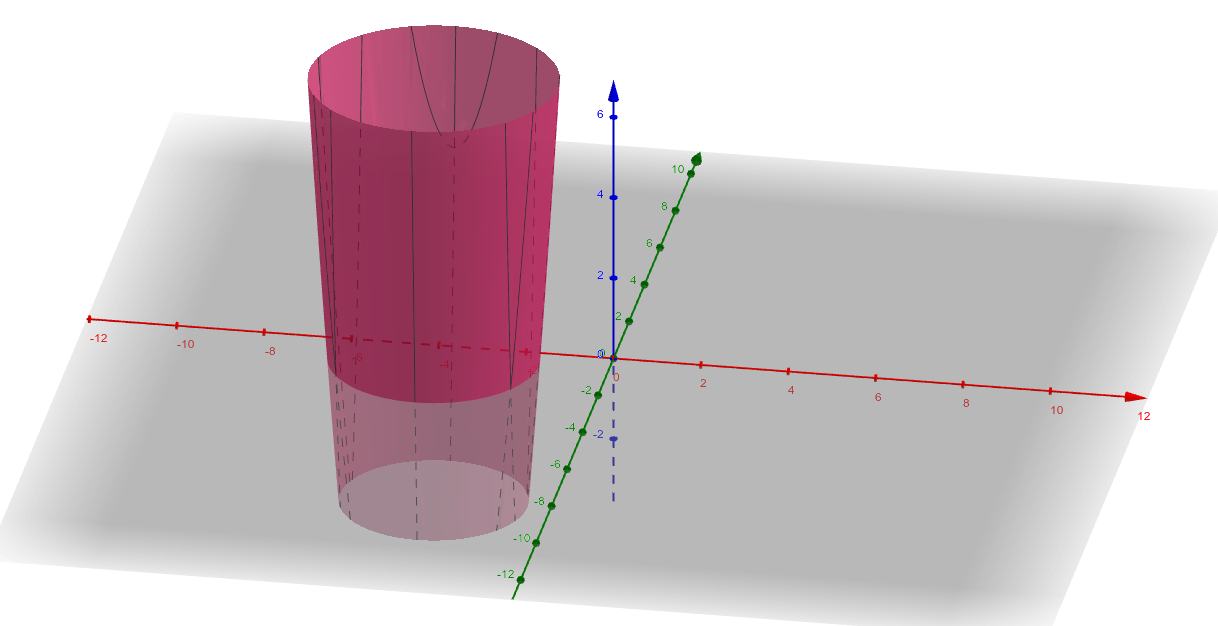
\includegraphics[scale=0.4]{ex4.png}
		\caption{}
		\label{fig:1}
	\end{figure}
    
\end{document}